\glsresetall

\chapter{Einleitung}

Dieses Kapitel befasst sich mit der Motivation, die sich hinter der Erforschung der API-Usability von SeqAn verbirgt. Es beantwortet die Fragen, was API-Usability überhaupt ist und weshalb sie so wichtig ist. Anschließend wird erläutert, worum es sich bei SeqAn exakt handelt, und welchen Zweck SeqAn erfüllt. Abgeschlossen wird dieses Kapitel mit der Vorstellung, der in dieser Arbeit verwendeten \glslink{gtm}{Grounded Theory Forschungsmethode}.



\section{Motivation}
\label{sec:motivation}

Diese Arbeit verfolgt das Ziel, die Benutzerfreundlichkeit\footnote{Die Übersetzung des englischen Begriffs \textit{Usability} ins Deutsche ist kompliziert. Nach dem Inhalt der DIN EN ISO 9241 müsste man den Begriff ``Gebrauchstauglichkeit'' verwenden, wohingegen --- nach meinem persönlichen Eindruck --- der Begriff ``Benutzerfreundlichkeit'' von der deutschen Bevölkerung besser verstanden und vorgezogen wird. Ich werde daher alle drei Begriffe synonym verwenden. In \sref{sec:def-usability} gehe etwas genauer auf dieses Problem ein.} (engl. \textit{Usability}) der Softwarebibliothek \textit{SeqAn} im Rahmen einer explorativen empirischen Fallstudie zu verbessern. Wie ich\footnote{Diese Arbeit ist in der Ich-Form verfasst. Die Begründung für diesen Entschluss ist in der verwendeten Forschungsmethode begründet, die ich ab Seite \pageref{sec:gtm} vorstelle.} im \hyperref[sec:forschungsstand]{nächsten Kapitel} noch erläutern werde, ist die klassische Usability-Verbesserung von Endanwender-Programmen bereits gut erforscht und, für sich genommen, lediglich anspruchsvolles Handwerk. Anders sieht es aus, wenn beispielsweise neuartige Bedienkonzepte entwickelt, evaluiert und verbessert werden sollen.

Im Falle von SeqAn sind gleich zwei Aspekte interessant:
\begin{enumerate}
  \item SeqAn ist keine Anwendersoftware, mit der durch eine \gls{gui} interagiert wird, sondern eine Softwarebibliothek, die mittels einer weiter unten definierten \glslink{api}{Applikationsprogrammierschnittstelle (engl. \textit{application programming interface}, kurz: API)} verwendet wird.
      \\Oder anders ausgedrückt: Während man in ``normalen Programmen'' herum klickt, muss man bei SeqAn mit Hilfe einer selbst gewählten Entwicklungsumgebung programmieren.
  \item SeqAn löst keine Informatik-eigenen Probleme wie Persistierung oder Logging, sondern bietet Funktionen zur Lösung von Problemen aus der Bioinformatik an. 
\end{enumerate}

Schaut man genauer hin, ergeben sich drei anspruchsvolle, zu lösende Problemfelder:
\begin{enumerate}
  \item Im Bereich der Forschung wurde der Usability von APIs weit weniger Aufmerksamkeit geschenkt, als der Usability von Endanwender-Programmen \citep{Grill:2012jm}. Erst seit Kurzem hat das Interesse an API-Forschung wegen des ansteigenden Gebrauchs von APIs zugenommen \citep{Daughtry:2009be}. 2009 fand das erste und bis dato einzige Treffen der \textit{Special Interest Group} ``API Usability'' auf der CHI 2009\footnote{\url{http://www.chi2009.org}} statt \citep{Daughtry:2009dv}. Wie ich im \hyperref[sec:forschungsstand]{nächsten Kapitel} zeigen werde, ist der Korpus an empirischer Grundlagenforschung klein und es fehlen umfassende wissenschaftliche Literaturstudien.
  \item SeqAns Alleinstellungsmerkmal ist seine kompromisslose Effizienz. Um diese zu erreichen, basiert SeqAn auf dem sehr anspruchsvollen Programmierparadigma \textit{Templatemetaprogrammierung}\footnote{Dass es sich bei der Templatemetaprogrammierung um die Hauptursache für SeqAns fragliche Usability handeln würde, schien allen Beteiligten mehr oder minder klar zu sein. Wenn ich im diesen Sinne von der Templatemetaprogrammierung spreche, handelt es sich allerdings um einen Vorgriff auf mein in dieser Arbeit vorgestelltes Forschungsergebnis. Bewusst habe ich auch andere Ursachen in Betracht gezogen, die ich ebenfalls in dieser Arbeit vorstelle.}, zu der es keinerlei Erkenntnisse in Bezug auf die Usability gibt.
  \item Das Spektrum an Anwendern von SeqAn ist breit und reicht vom professionellen Entwickler bis hin zum Biologen mit minimalen Programmierfertigkeiten. Letzterer gehört der Gruppe der \textit{Endanwender-Programmierer} an \citep{Tisdall:2001td}. Die Forschung im Bereich der Endanwender-Programmierung hat sich allerdings vornehmlich auf visuelle Programmiersprachen\footnote{Definition nach \cite{schiffer1998visuelle}: ``Eine visuelle Sprache ist eine formale Sprache mit visueller Syntax oder visueller Semantik und dynamischer oder statischer Zeichengebung.''} konzentriert \citep{Ko:2011el,Gieselmann:-Uisl6hs}, zu der die von SeqAn verwendete Programmiersprache C{}\verb!++! nicht gehört.
\end{enumerate}

Im Folgenden möchte ich klären, was Bioinformatik überhaupt ist, weshalb Bioinformatiker APIs benötigen und welchen Nutzen APIs im Speziellen wie auch im Allgemeinen haben. 



\subsection[Bedeutung der Bioinformatik]{Was ist überhaupt Bioinformatik?}

Die Bioinformatik ist eine interdisziplinäre Wissenschaft, die Methoden der Informatik auf biologische Daten und Fragestellungen anwendet \citep{Gibas:2002wk}. Quellen für biologische Daten sind dabei Sequenzierungen von Genomen, Expressionsprofile von Proteinen, Strukturaufklärung von Proteinen und Interaktionen zwischen Biomolekülen wie Proteinen, RNAs und niedermolekularen Verbindungen \citep{Rarey:E0TiqhGO}.

Mit jedem Jahr werden immer größere Datenmengen produziert. Allein das menschliche Genom umfasst etwa 3 Milliarden Basenpaare\footnote{Das Basenpaar beschreibt ein Paar Nukleobasen. Die wohl bekanntesten Basen sind \textbf{A}denin, \textbf{C}ytosin, \textbf{G}uanin und \textbf{T}hymin. Sie treten bei der DNA als die Paare A-T und C-G auf.} \citep{Tisdall:2001td}. Deutlich kleinere Genome können bei Auswertungszwischenschritten bereits mehrere Terabytes große Datenmengen verursachen \citep{Reinert:tg}. Der Zuwachs an Daten hat mittlerweile ein exponentielles Wachstum angenommen. Für die Vorbereitung, Auswertung und Analyse dieser Datenmassen werden Werkzeuge benötigt, die durch die Bioinformatik bereitgestellt werden \citep{Gibas:2002wk}.

Das Hauptaufgabengebiet der Bioinformatik liegt in der Sequenzanalyse. Darunter wird die Analyse von biomolekularen Sequenzen, wie der DNA, RNA oder Aminosäuren verstanden. Diesem Vorgehen liegt die Beobachtung zu Grunde, dass eine hohe Sequenzähnlichkeit für gewöhnlich eine signifikante, funktionale oder strukturelle Ähnlichkeit impliziert \citep{AlgorithmenundDate:2011wx}. Zu den ersten Bioinformatikern gehören \cite{Needleman:1970vq}, auf deren Algorithmus heute noch viele Methoden zur Sequenzanalyse basieren \citep{hansen2013bioinformatik}.

In den vergangenen Jahren sind die Kosten für Hochdurchsatz-Sequenzierungsverfahren, die auch als \textit{Next Generation Sequencing} (NGS) bezeichnet werden, rapide gefallen. Dies führt zu einer extrem schnellen Entwicklung im Feld der Bioinformatik \citep{Li:2012fl}. So haben beispielsweise \cite{Alexander:2012fb} ein Verfahren entwickelt, das einen potentiell vorliegenden Schilddrüsenkrebs ohne chirurgischen Eingriff mit hoher Wahrscheinlichkeit ausschließen kann. Dieses Verfahren kann Patienten die unnötige Entfernung ihrer Schilddrüse und die damit einhergehende lebenslange Hormontherapie ersparen.

Bereits heute ist die Sequenzierung eines menschlichen Genoms für weniger als 1.000\$ zu haben \citep{Young:2014tl}; in wenigen Jahren wird die 100\$-Grenze unterschritten sein \citep{Reinert:tg}. Diese Entwicklung ermöglicht vollkommen neue Anwendungsformen, z.B. in den Bereichen der personalisierten Medizin, Metagenomik und der klinischen Forschung \citep{Reinert:tg}. SAP-Mitgründer Dietmar Hopp spricht sogar davon, ``dass Life Sciences die nächste Welle nach der Informationsverarbeitung sein wird'' und hat bereits mehr als eine Milliarde Euro in den Bereich der Biotechnologie investiert \citep{Ziegler:2015tt}. Auf staatlicher Ebene werden, teil bereits seit Jahren, nationale Großprojekte verfolgt \citep{Young:2014tl}. Ein solches ist das \textit{Genomics England} Projekt\footnote{\url{http://www.genomicsengland.co.uk}}, das durch den staatlichen Gesundheitsanbieter \textit{National Health Service}\footnote{\url{http://www.nhs.uk}} geplant wird. Dieses Projekt sieht vor, bis 2017 die Gendaten von insgesamt 100.000 Patienten vollständig zu erfassen und in einem ersten Schritt für die Erforschung von seltenen Krankheiten, Krebs und Infektionskrankheiten zu nutzen.

Die auch als \textit{Bioethik} bezeichnete ethische Auseinandersetzung setzt sich in einer überraschenden Breite sowohl mit ganz grundsätzlichen \citep{Bouvet:2006ig}, wie auch methodischen \citep{Vayena:2015kk}, als auch didaktischen \citep{Gasparich:2014eg} Fragestellungen auseinander. Auch hoch aktuelle Themen, wie der immer noch andauernde Ebola-Ausbruch in Westafrika im Frühjahr 2014, sind Gegenstand des ethischen Diskurses \citep{Blais:2015tw}. Auf nationaler Ebene beschäftigt sich der Ethikrat der Bundesrepublik Deutschland auch mit der Bioethik\footnote{\url{http://www.ethikrat.org/veranstaltungen/anhoerungen/praediktive-genetische-diagnostik-multifaktorieller-erkrankungen}}. Auf internationaler Ebene ist dafür das bereits 1993 eingerichtete \textit{International Bioethics Committee}\footnote{\url{http://www.unesco.org/new/en/social-and-human-sciences/themes/bioethics/international-bioethics-committee/}} zuständig. 




\subsection[Bioinformatik und Programmieren]{Warum müssen Bioinformatiker und Biologen programmieren?}

Wie bereits erwähnt, entwickelt sich die Bioinformatik rasant. Während die Datenmengen stetig steigen, entstehen immer wieder neue Algorithmen und Hypothesen \citep{Letondal:2006dy}. Diese Entwicklung führt dazu, dass Probleme formuliert werden, für deren Lösung es noch keine \citep{Tisdall:2001td} oder nur unzureichende \citep{Letondal:2006dy} grafische Werkzeuge existieren.

Während es zu den fachbedingten Tätigkeiten der Bioinformatik gehört, Code schreiben zu müssen, trifft dies nun auch auf Biologen zu. Anders wäre es ihnen nicht möglich, neuartige Hypothesen zu überprüfen \citep{Letondal:2006dy,Tisdall:2001td}. Damit bilden Biologen klassische Vertreter der Endanwender-Programmierer.

Unabhängig von verfügbaren grafischen Werkzeugen gibt es einen immensen Automatisierungsbedarf in Form von Stapelverarbeitungsskripten (engl. \textit{batch scripts}) und \textit{Workflows}. Abgesehen von der geringeren Fehlerquote wird Automatisierung durch den enormen Zeitgewinn motiviert: Während die händische Auswertung von Gen-Abschnitten einen Monat oder mehr beanspruchen kann, kann ein in zwei Wochen entwickeltes Skript dieselbe Arbeit in 30 Minuten leisten \citep{Tisdall:2001td}. Bedenkt man das Alter der Quelle und die fortschreitende Entwicklung von Informatik und Bioinformatik, wird dieser Zeitgewinn sicherlich gewachsen sein.

Die Bioinformatik verfügt bereits über ein großes Repertoire an Algorithmen, die Lösungsbestandteile neuartiger Probleme darstellen. Existierende Implementierungen werden über Softwarebibliotheken, Frameworks, etc. bereitgestellt; sie wiederzuverwenden verringert die Anzahl an produzierten Defekten in den entwickelten Werkzeugen und erhöht zugleich die Effizienz der Arbeit.





\subsection[Relevanz von API-Usability]{Warum ist die Benutzerfreundlichkeit von APIs überhaupt so wichtig?}

Moderne Softwareentwicklung macht ausgiebig Gebrauch von dem Prinzip der Wiederverwendung \citep{Piccioni:2013uq}. Wiederverwendbarer Code wird am häufigsten in Form von \textit{Frameworks} und \textit{Softwarebibliotheken} bereitgestellt \citep{Henning:2007kg,Jeong:kf}, wobei letztere am häufigsten von Anwendern genutzt werden \citep{Feilkas:dg}. Die Nutzung von existierendem qualitativem Code hat gegenüber der Neuimplementierung potentiell die Vorteile geringerer Kosten sowie eine höhere Sicherheit und Stabilität \citep{Stylos:2009ts}.

Der Zugriff auf eine Softwarebibliothek wird über eine API realisiert. Weil es sich dabei um die Schnittstelle zwischen Anwender und Softwarebibliothek handelt, ist die Usability ein fundamentales Ziel bei der Entwicklung der API \citep{Piccioni:2013uq}.

APIs sind schwer zu verwenden \citep{Stylos:2006ji} und schwer zu erlernen, weil nicht nur die einzelne Klasse, sondern auch das Zusammenspiel der Klassen wichtig ist \citep{Bruch:2006bv}. Das gilt sogar für etablierte APIs wie dem Java Development Kit\footnote{\url{http://www.oracle.com/technetwork/java/javase}} \citep{Stylos:2009gc}. In besonders schweren Fällen kann der Verwender einer API sogar so stark ausgebremst werden, dass er schneller ohne die Verwendung der API gewesen wäre \citep{Stylos:2007ip}.

Eine schlechte API-Usability verringert die Produktivität und Codequalität \citep{Zibran:2011fx} bei der Entwicklung von Programmen mit Hilfe dieser API. Inzwischen ist eine \textit{API-Ökonomie} entstanden \citep{Hulsenbusch:2014wr}, bei der sich die Benutzerfreundlichkeit natürlich auch auf die Wettbewerbsfähigkeit auswirkt \citep{Stylos:2009ts}. Ist eine API zu schwer zu erlernen, wechseln die Anwender eben auf eine andere API \citep{sunshine2014searching}. Aus humanistischer und arbeitspsychologischer Sicht wirkt sich die Arbeit mit einem benutzer\textit{un}freundlichen System negativ auf Wohlbefinden und Motivation aus \citep{Sarodnick:2006vc}.

\subsection[Nutzen von API-Usability]{Lohnt sich wirklich der Aufwand zur Verbesserung der Benutzerfreundlichkeit von APIs?}

Diese Frage ist nicht nur für die Leser und Geldgeber dieser Arbeit sowie für die Autoren von APIs von Wichtigkeit, sondern auch für mich selbst. Schließlich stand ich vor der Wahl, eine Promotion über einen Zeitraum von drei oder mehr Jahren zu verfolgen und fachlich wie auch motivatorisch zu meistern.

Etablierte APIs werden tausendfach häufiger verwendet als entwickelt \citep{Ellis:2007kv}. Die Mehrkosten für die Autoren von APIs sind vielfach kleiner als der Schaden, den benutzerunfreundliche APIs ihren Anwendern anrichten \citep{Henning:2007kg}. Die Verantwortung für eine benutzerfreundliche API liegt also klar bei seinen Autoren. Außerdem ist eine einmal veröffentlichte API quasi ewig --- es existiert also nur eine Chance, sie korrekt zu entwerfen \citep{Bloch:2006jk}.

Wird die API-Usability nicht explizit beim Entwurf beachtet, ist sie weiter nichts als ein extrem unwahrscheinlicher Zufall \citep{Stylos:2009ts}. Bereits kleine und unschuldig anmutende Mängel tendieren dazu, sich negativ in überproportionalen Größenordnungen auszuwirken \citep{Henning:2009hz}. \cite{Stylos:2007ip} bezeichnen dies trefflich als ``death by 1000 paper cuts''.

Für die besonders anspruchsvolle Anwendergruppe der Endanwender-Programmierer, zu denen auch Biologen \citep{Tisdall:2001td} und teilweise auch Bioinformatiker \citep{Letondal:2006dy} gehören, ist das Schadpotential besonders groß. Schließlich verfügt diese Gruppe über weit weniger Erfahrung im Bereich der Softwaretechnik und kann Usability-Probleme weniger gut kompensieren, als ihre erfahreneren Kollegen \citep{Shaft:1998tc}.

Die Verbesserung der API-Usability ist möglich und wurde in einigen Studien gezeigt \citep{Letondal:2006dy,Grill:2012jm,Tenny:2011jp,Piccioni:2013uq}. Wie meine, im \sref{sec:forschungsstand} vorgestellte Literaturrecherche zeigt, ist der Wissensstand in diesem Bereich jedoch noch stark fragmentiert. Ein Grund dafür ist --- neben der Vernachlässigung von API-Usability zu Gunsten der klassischen Usability --- die Vielzahl an Einflussfaktoren, zu denen, neben der API selbst, auch die dazugehörige Dokumentation, die gewählte Programmiersprache und Entwicklungswerkzeuge gehören \citep{Stylos:2008jt}.

\subsection{Synthese und Zusammenfassung}

APIs bilden die Schnittstelle zu wiederverwendbarem Code. Ohne diese Schnittstelle ist der Nutzer gezwungen, Code zu duplizieren, was zu einer ganzen Fülle von Nachteilen führt \citep{Spinellis:2006tj}. Glücklicherweise wird wiederverwendbarer Code häufig in Form von Softwarebibliotheken gekapselt und durch APIs zugänglich gemacht.

Eine benutzerunfreundliche API führt zu einer Reihe von Problemen, die sich negativ auf die ganze Spannbreite von persönlichen bis hin zu wirtschaftlichen Erfolgsfaktoren auswirken. Um diesen potentiellen Schaden abzuwenden, müssen sich die Entwickler einer API aktiv für dessen Usability einsetzen. Bei ihnen liegt aus fachlichen und ökonomischen Gründen die Verantwortung dafür. Leider ist diese Anforderung leichter formuliert als erfüllt, denn die Forschung im Bereich der API-Usability steht der Forschung im Bereich der klassischen Usability um einiges nach. Hinzu kommt, dass es an umfassenden wissenschaftlichen Literaturstudien fehlt.

Die Bioinformatik entwickelt Werkzeuge, mit denen Problemstellungen gelöst werden können, die unter anderem zu einem besseren Verständnis von Krankheiten und deren Heilungsmöglichkeiten führen. Dazu greifen Bioinformatiker auf Softwarebibliotheken zurück. Eine solche Softwarebibliothek ist SeqAn, die das Leben ihrer Anwender durch den intensiven Gebrauch des Programmierparadigmas Templatemetaprogrammierung nicht unbedingt leicht macht. Zu allem Überfluss ist dieses Paradigma in Bezug auf seine Benutzerfreundlichkeit vollkommen unerforscht.

Die allgemein formulierten Nachteile einer schlechten API-Usability bedeuten für den Bereich der Bioinformatik, dass die Forschung im besten Fall ausgebremst wird. Eine gute API-Usability hingegen erlaubt es nicht nur Bioinformatikern effizienter zu arbeiten, sondern kann --- unter Berücksichtigung von Erkenntnissen aus der Endanwender-Softwaretechnik --- Biologen in den Zustand versetzen, sich ebenfalls bioinformatisch zu betätigen. Dass dies tatsächlich möglich ist, konnte in einer Arbeit gezeigt werden \citep{Letondal:2006dy}, die ich im \sref{sec:letondal} vorstelle.

\bigskip

Als Forscher und Autor dieser Dissertation beschäftige ich mich also mit den Aufgaben, (1) eine umfassende wissenschaftliche Literaturstudie durchzuführen, (2) die Usability von Templatemetaprogrammierung im Allgemeinen und von SeqAn im Speziellen empirisch zu erforschen, (3) die besonderen Anforderungen von Endanwender-Programmierern zu berücksichtigen, (4) Vorschläge für die Verbesserung der Usability von SeqAn zu formulieren und (5) diese umzusetzen.





\section{Definitionen}
\label{sec:definitions}

An dieser Stelle möchte ich knapp auf Übersetzungsschwierigkeiten vom Englischen ins Deutsche eingehen: Bekanntermaßen ist die Informatik durch englischsprachige Begriffe geprägt. Außerdem wird der mit Abstand größte Teil wissenschaftlicher Veröffentlichungen im Bereich der Informatik in englischer Sprache verfasst. Für viele englische Begriffe gibt es etablierte Übersetzungen (z.B. \textit{interface} \& \textit{Schnittstelle}). Andere Begriffe lassen sich hingegen nur mühselig (z.B. \textit{usability} \& \textit{Gebrauchstauglichkeit}/\textit{Nutzbarkeit}/\textit{Benutzerfreundlichkeit}) oder gar missverständlich (z.B. \textit{framework} \& \textit{Rahmenwerk}) übersetzen.

Aus diesen Gründen werde ich für den Rest dieser Arbeit nach Möglichkeit den deutschen Begriff verwenden. Würde eine Übersetzung jedoch unnötig kompliziert sein oder gar missverstanden werden können, verwende ich den englischen Begriff. Wenn es sich um kein direktes Zitat handelt, schreibe ich englische Substantive mit großem Anfangsbuchstaben und verwende den sächlichen Artikel. Bei Abkürzungen, die sowohl den englischen als auch deutschen Begriff beschreiben (z.B. \textit{API}), nutze ich den Artikel des deutschen Begriffs (z.B. \textit{die API}). Von diesen Vereinbarungen mache ich gleich bei der folgenden ersten Definition Gebrauch.

\bigskip

Basierend auf existierenden Definitionen \citep{dekel2011increasing,Tenny:2011jp,zibran2008makes,Zibran:2011fx,McLellan:1998cu,Henning:2007kg,Robillard:2009cs,Stylos:2009ts}, definiere ich \textit{API} wie folgt:
\begin{description}
  \item Eine \glslink{api}{\textit{Applikationsprogrammierschnittstelle} (engl. \textit{application programming interface}, kurz: \textit{API})} ist eine Schnittstelle zwischen Anwender und dem der Schnittstelle zu Grunde liegenden Code, der eine bestimmte Funktionalität implementiert. Eine API liegt in Gestalt einer Softwarebibliothek, eines Framework, SDKs, Toolkits, etc. vor, umfasst alle dazu in Verbindung stehenden Ressourcen (Installationsdateien, Dokumentation, etc.) und definiert dabei eine Dienstleistung, welche die Komplexität der Implementierung mittels Abstraktion versteckt. Bei APIs handelt es sich um eine fortgeschrittene Form der Code-Wiederverwendung, die den Bau komplexer Software ermöglicht.
\end{description}

\bigskip

Obwohl es eine Reihe Veröffentlichungen im Bereich der API-Usability gibt, hat sich erstaunlicherweise noch keine grundlegende einheitliche Terminologie für die folgenden drei relevanten Parteien entwickelt. Einige Arbeiten verwenden zumindest den Begriff \textit{API user} --- ohne ihn jemals explizit eingeführt zu haben. Ich schlage daher folgende Begriffe vor:

\begin{description}
  \item Ein \textit{API-Entwickler} (engl. \textit{API developer} bzw. \textit{API designer}) ist eine Person, die an der Entwicklung einer API beteiligt ist. Neben der eigentlichen Programmierung gehören auch Konzeption, Entwurf oder Wartung in ihre Arbeitsbereiche.
  \item Ein \textit{API-Anwender} (engl. \textit{API user}) ist eine Person, die eine oder mehrere \glslink{api}{APIs} nutzt, um ein Problem programmatisch zu lösen.
\end{description}

\bigskip

Da sich diese Arbeit mit einer Software befasst, die nicht ausschließlich von professionellen Softwareentwicklern genutzt wird, muss sie sich auch mit der Endanwender-Softwaretechnik auseinandersetzen. \sref{sec:euse} befasst sich näher mit diesem Thema. An dieser Stelle möchte ich lediglich den Begriff des \textit{Endanwender-Programmierers} herausgreifen.

\begin{description}
  \item Ein \textit{Endanwender-Programmierer} (engl. \textit{end-user programmer}) ist eine Personen, deren Ziel --- im Gegensatz zum professionellen Programmierer --- nicht das Programmieren selbst ist. Stattdessen ist Programmieren für sie ein ``notwendiges Übel'' zur Erreichung ihres Ziels innerhalb ihrer Expertendomäne.
\end{description}

\bigskip

Auf den Bereich der API-Usability übertragen, können API-Entwickler und API-Anwender um eine weitere Rolle ergänzt werden:

\begin{description}
  \item Ein \textit{API-Endanwender} (engl. \textit{API end-user}) ist ein spezieller Endanwender-Programmierer, der eine API zum Erreichen seines Ziels nutzt.
\end{description}

Abhängig vom Kontext verwende ich den Begriff \textit{API-Anwender} als Überbegriff für \textit{API-Anwender} und \textit{API-Endanwender} --- also als undifferenzierte Bezeichnung für alle Anwender einer API.

\begin{comment}
\bigskip

Abschließend definiere ich noch die Rolle, die in der klassischen Usability-Forschung die sicherlich wichtigste Partei darstellt:

\begin{description}
  \item Ein \textit{Produkt-Anwender} bzw. \textit{Anwender} (engl. \textit{user}) ist eine Person, die durch API-Anwender erstellte Programme nutzt.
\end{description}

Es ist wichtig, diese Gruppe explizit zu benennen, da sie die Folgen einer guten bzw. schlechten API-Usability spürt. Bei APIs für grafische Benutzeroberflächen wie Swing, QT oder SWT ist dies besonders der Fall, da eine inkorrekte Verwendung dieser APIs sich besonders schnell in der grafischen Benutzeroberfläche des Endanwender-Programms bemerkbar macht.
\end{comment}

\bigskip

Wie ich weiter unten noch erläutern werde, ist die dieser Arbeit zu Grunde liegende Forschungsmethode die \textit{\gls{gtm}}. Diese Methode verwendet den englischen Begriff \textit{Code}, der leider mit dem Code-Begriff aus der Informatik kollidiert. Für den Rest dieser Arbeit werde ich für den GTM-Code-Begriff \textit{Kode} bzw. \textit{Konzept} und für den Informatik-Code-Begriff \textit{Code} bzw. \textit{Quellcode} benutzen.

Leider steht der GTM-Konzept-Begriff wiederum im Konflikt mit dem Konzept-Begriff aus der Templatemetaprogrammierung. Daher werde ich für den GTM-Konzept-Begriff \textit{Konzept} und für den Templatemetaprogrammierungs-Konzept-Begriff \textit{Concept} verwenden. Die Eselsbrücke lautet: Für nicht-technische Gebiete verwende ich die deutsche Übersetzung und für technische Konfliktbegriffe das englische Wort im Original.




\section{SeqAn}

SeqAn\footnote{\textbf{Seq}uenz-\textbf{An}alyse} ist eine quelloffene C{}\verb!++!-Softwarebibliothek, die von Andreas Gogol-Döring im Rahmen seiner Dissertation \citep{GogolDoring:2009vz} entwickelt wurde. Sie dient ihren Anwendern zur ``Verarbeitung großer Mengen biomedizinischer Daten, insbesondere von Gen- und Proteinsequenzen'' und mir als Forschungsgegenstand für API-Usability.

\bigskip

Typische Anwendungen sind \citep{Reinert:tg}:
\begin{description}\itemsep1pt\parskip0pt\parsep0pt
  \item[Indices] \hfill \\ Suche von Mustern in Sequenzen
  \item[Alignment] \hfill \\ Lokaler, globaler, semi-globaler, approximativer, etc. Vergleich von zwei oder mehr Sequenzen
  \item[Read-Mapping] \hfill \\ Zusammensetzung einer in vielen Fragmenten (engl. \textit{reads}) vorliegenden Sequenz
  \item[Assemblies] \hfill \\ Auffinden von genomischen Varianten
\end{description}

\bigskip

Bei der Entwicklung von SeqAn hatte \cite{GogolDoring:2009vz} zwei Anwendergruppen im Auge:
\begin{description}\itemsep1pt\parskip0pt\parsep0pt
  \item[Softwareentwickler,] die, neue Softwarewerkzeuge für die biologische und medizinische Forschung entwickeln und
  \item[Algorithmendesigner,] die neue Algorithmen entwickeln, testen und vergleichen wollen.
\end{description}

\bigskip

Für die Verwendung von SeqAn stehen zwei Möglichkeiten zur Verfügung: Einerseits kann SeqAn als Softwarebibliothek verwendet werden. Dieser Anwendungsfall ist der von mir in dieser Arbeit beleuchtete. Andererseits gibt es die Möglichkeit, die im \sref{sec:seqan-tools} beschriebenen und auf SeqAn basierenden Werkzeuge zu nutzen --- dieser Anwendungsfall wird in dieser Arbeit nicht beleuchtet, da es dabei nicht um \glslink{api}{API}-, sondern um klassische Usability geht.

Die immer größeren Datenmengen erfordern automatisierte Analyseverfahren, die eine hohe Sorgfalt und Verfahrenssicherheit aufweisen. Die wiederum stetig fallenden Sequenzierungskosten machen solche Verfahren auch für kleinere Pharmafirmen und Labore interessant \citep{Reinert:tg}. Für diese Anwendergruppe ist der Einsatz von SeqAn besonders interessant.

Bei der quelloffenen, freien Bereitstellung der Bibliothek gestaltet sich die Monetarisierungsform, die auf den Verkauf von Nutzungslizenzen setzt, schwierig. Daher setzen die SeqAn-Entwickler auf ein Beratungsmodell, bei dem die Nutzung von SeqAn kostenlos ist und die Möglichkeit besteht, beratende und entwickelnde Tätigkeiten kostenpflichtig in Anspruch zu nehmen.
 
\begin{figure}
  \centering
    
\includegraphics[width=0.35\linewidth]{Figures/seqan-logo.png}
  \caption[SeqAn-Logo]{Logo der Softwarebibliothek \textit{SeqAn}}
  \label{fig:seqan-logo}
\end{figure}


\subsection{Entwurf}
\label{sec:seqan-entwurf}

SeqAn wurde mit dem Ziel entwickelt, eine hohe Performanz, Allgemeingültigkeit, Erweiterbarkeit und Integration mit anderen Bibliotheken zu garantieren und dabei benutzerfreundlich zu sein \citep{GogolDoring:2009vz,gogol2009biological}. In die Entwicklung von SeqAn sind circa 18 Personenjahre investiert worden \citep{Reinert:tg}. Wie man unschwer erahnt, wird diese Arbeit zeigen, dass es um die Benutzerfreundlichkeit nicht gut bestellt ist.

Die größte Auffälligkeit beim Entwurf von SeqAn ist, dass auf objektorientierte Programmierung zu Gunsten von Templatemetaprogrammierung verzichtet wird. Der Entwicklung von SeqAn liegen vier von \cite{GogolDoring:2009vz} als ``Techniken'' beschriebene Entwurfsansätze zu Grunde:
\begin{description}
  \item[Generische Programmierung] \hfill \\
  SeqAn setzt generische Programmierung ein --- ein Paradigma, das auch der \textit{C{}}\verb!++! \textit{Standard Template Library} (\textit{STL}) zu Grunde liegt \citep{plauger2001c++}. Bei diesem Ansatz werden Algorithmen und Datenstrukturen derart entworfen, dass sie auf allen Datentypen operieren, welche die an sie gestellten Minimalanforderungen erfüllen.
  
  \item[Template-Subclassing] \hfill \\
  Diese Technik wird verwendet, um in SeqAn Polymorphismus zu ermöglichen. Dazu erhalten Klassen (z.B. \mintinline{cpp}{Class}) mindestens einen Templateparameter \mintinline{cpp}{TSpec}, mit dessen Hilfe dann Verfeinerungen beliebiger Tiefe vorgenommen werden können (z.B. \mintinline{cpp}{Class<SubClass>}, aber auch \mintinline{cpp}{Class<SubClass<SubSubClass>>}). Dies ermöglicht es, spezialisierte generische Funktionen für bestimmte Eingaben bereitzustellen, die ein Problem effizienter lösen, als dies die Standardimplementierung zulässt.
  
  Gepaart mit der generischen Programmierung führt diese Technik zu höchst performanten Programmen, denn die korrekte Implementierung für einen Funktionsaufruf wird zur Kompilier- und nicht zur Laufzeit ermittelt.
  
  \item[Globales Funktionen-Interface] \hfill \\
  Dieser Ansatz ist mehr eine Notwendigkeit als ein Feature, denn der Einsatz von Template-Subclassing erfordert die Bereitstellung aller verfeinerbaren Funktionen in einem gemeinsamen Namensraum, was in globalen Funktionen resultiert. Damit verlieren die Funktionen technisch gesehen ihre Zugehörigkeit zu einer Klasse. Semantisch existiert diese Zugehörigkeit dennoch. Die semantisch zu einem Typ gehörenden Funktionen werden als globales Funktionen-Interface bezeichnet. Anstatt also \mintinline{cpp}{obj.fn()} aufzurufen, müssen API-Anwender \mintinline{cpp}{fn(obj)} verwenden.
  
  Für die API-Anwender ergeben sich Probleme, die entweder zu Stande kommen, weil eine Funktion aufrufbar ist, die für den in Frage stehenden Typ eigentlich gar nicht definiert sein sollte (z.B. die \mintinline{cpp}{length}-Funktion\footnote{\url{http://docs.seqan.de/seqan/develop/?p=ContainerConcept\#length}}) oder weil gleichnamige Funktionen --- abhängig von ihrer Eingabe --- nun plötzlich vollkommenen verschiedene Dinge erledigen (z.B. die \mintinline{cpp}{label}-Funktion\footnote{\url{http://docs.seqan.de/seqan/develop/?p=Fragment\#label} bzw.\\\url{http://docs.seqan.de/seqan/develop/?p=EdgeIterator\#label}}). Die Folgen werden ausführlich in den Ergebnissen in \href{sec:gt}{Kapitel 4} erläutert.
  
  Um die Kompatibilität zu anderen Bibliotheken, wie der \textit{C{}}\verb!++! \textit{Standard Library} (\textit{STD}), herzustellen, werden \textit{Shims} verwendet. Dabei handelt es sich um globale Funktionen, welche die existierenden Memberfunktionn einfach durch einen entsprechenden Funktionsaufruf kapseln. Beispiel: Die Funktionen des globalen Funktionen-Interfaces für SeqAn-Strings können auch auf C{}\verb!++!-Strings operieren, indem sie auf die jeweilige Memberfunktionen des C{}\verb!++!-Strings zugreifen. Das globale \mintinline{cpp}{length}-Shim für C{}\verb!++!-Strings wurde wie folgt implementiert, wobei der relevante Aufruf in Zeile 6 stattfindet:

\begin{minted}[linenos=true, firstnumber=1, autogobble=false]{cpp}
template <typename TChar, typename TCharTraits, typename TAlloc>
inline typename Size< std::basic_string<TChar, TCharTraits, TAlloc> >::Type
length(std::basic_string<TChar, TCharTraits, TAlloc> const &me)
{
    SEQAN_CHECKPOINT;
    return me.length();
}
\end{minted}
  
  \item[Metafunktionen] \hfill \\
  Metafunktionen sind Funktionen, die nicht zur Lauf-, sondern zur Kompilierzeit ausgeführt werden. In SeqAn werden sie hauptsächlich dazu verwendet, zu einem gegebenen Eingabetyp den dazugehörigen Ausgabetyp zu berechnen. Dieser Ansatz findet beispielsweise bei der Erzeugung von Iteratoren Anwendung, denn der Typ des Iterators hängt von der Eingabe der erzeugenden Laufzeit-Funktion \mintinline{cpp}{begin} ab\footnote{\url{http://docs.seqan.de/seqan/develop/?p=ContainerConcept\#begin}}. Implementiert werden Metafunktion in SeqAn mittels Klassentemplates. Das folgende Beispiel zeigt die Anwendung der Metafunktion \mintinline{cpp}{Iterator} in den Zeilen 2 und 3:

\begin{minted}[linenos=true, firstnumber=1, autogobble=true]{cpp}
    Dna5String genome = "TATANNNGCGCG";
    Iterator<Dna5String>::Type it = begin(genome);
    Iterator<Dna5String>::Type itEnd = end(genome);

    while (it != itEnd)
    {
        std::cout << *it;
        ++it;
    }
    std::cout << std::endl;
\end{minted}
  
  \item[Tag Dispatching] \hfill \\
  Mit Hilfe der generischen Programmierung und dem Template-Subclassing ist ein \textit{C{}}\verb!++!-Compiler in der Lage, die passendste Implementierung für einen Funktionsaufruf zur Kompilierzeit zu ermitteln. Allerdings möchte man auf diesen Prozess, beispielsweise bei der Wahl zwischen alternativen Alignment-Algorithmen, Einfluss nehmen können. Dazu kann der entsprechenden Funktion ein sogenannter, als Member-lose Klasse implementierter, \textit{Tag} übergeben werden. Für die Auswahl einer Alignment-Implementierung stehen beispielsweise \mintinline{cpp}{NeedlemanWunsch} und \mintinline{cpp}{MyersHirschberg} zur Verfügung.
\end{description}



\subsection{Beispiel}

Um den obigen technischen Erläuterungen ein wenig Leben einzuhauchen, stelle ich an dieser Stelle ein typisches, knappes SeqAn-Programm vor und wie dessen Entsprechung in Java aussehen könnte. Das Beispiel soll einerseits dabei helfen, einen besseren Eindruck von der Gestalt von auf SeqAn basierenden Programmen zu bekommen. Andererseits soll es das Verstehen dieser Arbeit erleichtern, weil ich immer wieder auf die Entwurfsentscheidungen von SeqAn zu sprechen kommen werde und diese in der Vorstellung meiner Analyseergebnisse eine große Rolle spielen.

Das folgende Programm berechnet das Alignment von zwei DNA-Sequenzen und gibt die Abweichung (\textit{Score}), eine textgrafische Darstellung und die reverse DNA-Sequenz der ersten Sequenz aus:

\begin{center}
\begin{minted}[linenos, firstnumber=1, autogobble=true]{cpp}
int main()
{
    typedef String<Dna> TSequence;
    typedef Align<TSequence, ArrayGaps> TAlign;
    
    TSequence seq1 = "ATAAGCGTCTCG";
    TSequence seq2 = "TCATAGAGTTGC";

    TAlign align;
    resize(rows(align), 2);
    assignSource(row(align, 0), seq1);
    assignSource(row(align, 1), seq2);
    
    int score = globalAlignment(align, Score<int, Simple>(0, -1, -1));
    std::cout << "Score: " << score << std::endl;
    std::cout << align << std::endl;
    
    std::cout << "Complement of sequence #1: ";
    Iterator<TSequence, Rooted>::Type it = end(seq1);
    for (goEnd(it); !atBegin(it); goPrevious(it))
    {
        std::cout << getValue(it);
    }
    std::cout << std::endl;
    return 0;
}    
\end{minted}
\captionof{listing}[Beispiel: Typisches SeqAn-Programm]{Beispiel --- Typisches SeqAn-Programm.

\textbf{Template-Subclassing:} In Zeile 3 wird eine Spezialisierung der String-Klasse speziell für Nukleotide definiert. In Zeile 4 wird die Datenstruktur definiert, die sowohl als Ein- als auch Ausgabe für die Berechnung des Alignments in Zeile 14 dient. Der zweite Template-Parameter spezifiziert, in welcher Weise das Alignment intern dargestellt wird. Diese Wahl beeinflusst das Laufzeitverhalten für bestimmte Operationen. \textbf{Globales Funktionen-Interface:} In den Zeilen 11 und 12 wird die globale \mintinline{cpp}{assignSource}-Funktion verwendet, die semantisch eine Memberfunktion der \mintinline{cpp}{Align}-Klasse ist.\footnote{Tatsächlich ist die \mintinline{cpp}{assignSource}-Funktion eine Memberfunktion der \mintinline{cpp}{Gaps}-Klasse, was an dieser Stelle aber nicht zum Verständnis beiträgt.} Im Gegensatz dazu ist die \mintinline{cpp}{globalAlignment}-Funktion technisch, wie auch semantisch, globale. \textbf{Generische Programmierung:} Die \mintinline{cpp}{resize}-Funktion in Zeile 10 ist ein hervorragendes Beispiel, denn sie operiert auf jeder Eingabe, deren Größe verändert werden kann. Tatsächlich ist das gesamte Programm generisch. Schließlich kann das Alignment für beliebige Elemente berechnet werden, wenn \mintinline{cpp}{String} in Zeile 3 entsprechend spezialisiert wird und der dort angegebene Datentyp den Gleichheitsoperator unterstützt. In Zeile 19 wird die \textbf{Metafunktion} \mintinline{cpp}{Iterator} aufgerufen. Diese Funktion gibt ein \mintinline{cpp}{struct} mit dem Feld \mintinline{cpp}{Type} zurück, das den Datentyp enthält, der einen Iterator für \mintinline{cpp}{TSequence} speichern kann. Das Wissen um die konkrete Implementierung der \mintinline{cpp}{Iter}-Klasse ist nicht nötig.}
\label{lst:seqan-typical}
\end{center}

\bigskip

Würde man das obige Programm 1:1 nach Java übersetzen, würde das Programm in etwa wie folgt aussehen:

\begin{center}
\begin{minted}[linenos, firstnumber=1, autogobble=true]{java}
private static class TSequence extends String<Dna> {};
private static class TAlign extends Align<TSequence, ArrayGaps> {};

public static void main(String[] args) {
    TSequence seq1 = new TSequence("ATAAGCGTCTCG");
    TSequence seq2 = new TSequence("TCATAGAGTTGC");

    TAlign align = new TAlign();
    align.setSize(2);
    align.getRows().assignSource(seq1, 0);
    align.getRows().assignSource(seq2, 1);

    int score = Alignment.globalAlignment(align, new Score<Integer, Simple>(0, -1, -1));
    System.out.println("Score: " + score);
    System.out.println(align);

    System.out.print("Complement of sequence #1: ");
    for(Iterator<TSequence, Rooted> iterator = seq1.end(); iterator.hasPrevious();) {
        System.out.print(iterator.prev());
    }
    System.out.print("\n");
}
\end{minted}
\captionof{listing}[Beispiel: Typisches SeqAn-Programm in Java I]{Beispiel --- Unmittelbare Übersetzung eines typischen SeqAn-Programms in Java}
\label{lst:seqan-typical-java1}
\end{center}

\bigskip

Die unmittelbare Java-Übersetzung wirkt etwas künstlich. Ein Java-Entwickler würde wahrscheinlich die folgende mittelbare Variante als die für ihn am vertrautesten empfinden:

\begin{center}
\begin{minted}[linenos, firstnumber=1, autogobble=true]{java}
public static void main(String[] args) {
    String<Dna> seq1 = new String<Dna>("ATAAGCGTCTCG");
    String<Dna> seq2 = new String<Dna>("TCATAGAGTTGC");

    Align<String<Dna>, ArrayGaps> align = new Align<String<Dna>, ArrayGaps>(seq1, seq2);

    int score = Alignment.computeGlobalAlignment(align, new Score<Integer, Simple>(0, -1, -1));
    System.out.println("Score: " + score);
    System.out.println(align);

    System.out.print("Complement of sequence #1: ");
    Iterator<String<Dna>> iterator = seq1.iterator(seq1.size());
    while(iterator.hasPrevious()) {
        System.out.print(iterator.previous());
    }
    System.out.print("\n");
}
\end{minted}
\captionof{listing}[Beispiel: Typisches SeqAn-Programm in Java II]{Beispiel --- Mittelbare Übersetzung eines typischen SeqAn-Programms in Java}
\label{lst:seqan-typical-java2}
\end{center}

\bigskip

Wie man an der Java-Übersetzung sehen kann, unterscheidet sich die Programmierung mit SeqAn deutlich von der objektorientierten Programmierung. In \href{sec:gt}{Kapitel 4} diskutiere ich die sich daraus ergebenden Probleme. Ursachen sind insbesondere die technische Auflösung von Memberfunktionen durch die Verwendung von generischer Programmierung im Zusammenspiel mit dem globalen Funktionen-Interface (siehe \sref{sec:lie-oop}) und der intensive Gebrauch von Metafunktionen (siehe \sref{sec:lie-usability}), welche von den SeqAn-Anwendern nur unzureichend verstanden werden.

Die im Zuge dieser Arbeit umgesetzten und in \sref{sec:seqan-api-usability-verbesserung} vorgestellten API-Usability-Verbesserungen umfassen ein Tutorial\footnote{\url{http://seqan.readthedocs.org/en/master/Tutorial/FirstStepsInSeqAn.html}}, das sich explizit an SeqAn-Anfänger richtet. Der gewillte Leser erfährt dort noch detaillierter, weshalb und wie die eben beschriebenen vier Grundtechnologien in SeqAn eingesetzt werden.



\subsection{Bestandteile}

Die Softwarebibliothek SeqAn besteht aus den im Folgenden vorgestellten Komponenten:

\subsubsection{Softwarebibliothek}
Die herunterladbare Softwarebibliothek, ist das, was man unter SeqAn im engeren Sinne versteht. Dabei handelt es sich um eine Archiv-Datei, die zur Verwendung entpackt werden muss. Das so entstehende SeqAn-Verzeichnis enthält die SeqAn-Quellen und insbesondere die \texttt{seqan.h}-Header-Datei, die in das eigene Softwareprojekt eingebunden werden kann.

Ursprünglich war SeqAn --- entgegen seines Namens --- nur als Framework nutzbar, was Usability-Probleme zur Folge hatte. Auf diese Beobachtung gehe ich in den Abschnitten \ref{sec:library-vs-framework} und \ref{sec:lie-library} ein.

\subsubsection{Website}

Die SeqAn-Website \url{http://www.seqan.de} ist der erste Anlaufpunkt für SeqAn-Anwender. Die Website informiert über Neuigkeiten rund um SeqAn, bietet Download-Möglichkeiten für die Bibliothek selbst und Anwendungen an und verweist auf alle weiter unten aufgeführten Ressourcen.

\subsubsection{Dokumentation}

Die Dokumentation umfasst im engeren Sinne die Beschreibungen der Klassen, Metafunktionen, Funktionen, etc., die von SeqAn bereitgestellt werden. Ursprünglich basierte sie auf der eigens für SeqAn entwickelten Dokumentationssprache \textit{DDDoc} \citep{GogolDoring:2009vz}. Die Dokumentation wurde im Zuge dieser Arbeit jedoch auf eine standardkonformere Eigenentwicklung umgestellt, was im \sref{sec:dox} ausführlich erklärt wird.

Die Dokumentation ist Bestandteil der herunterladbaren Archiv-Datei, kann jedoch auch Online unter \url{http://docs.seqan.de} konsultiert werden. Unter dieser Adresse stehen auch Revisionen zu den Major-Releases von SeqAn bereit.

Im weiteren Sinne umfasst die Dokumentation auch die sogenannten \textit{Tutorials}.

\subsubsection{Tutorials}

Tutorials\footnote{Eigentlich gibt es für den englischen Begriff \textit{Tutorial} die deutsche Übersetzung \textit{Tutorium}. Der englischsprachige Begriff \textit{Tutorial} ist jedoch derart im Vokabular der SeqAn-Entwickler und -Anwender verwurzelt, dass ich diesen Begriff dem deutschen ebenfalls vorziehe.} sind unter \url{http://seqan.readthedocs.org} konsultierbare Anleitungen für die verschiedenen SeqAn-Funktionen. Die Spannbreite reicht von Installationanleitungen über den Gebrauch von Iteratoren bis hin zum Alignment mehrerer Sequenzen.

Die Tutorien wurden ursprünglich über eine selbst verwaltete \textit{trac}\footnote{\url{http://trac.edgewall.org}}-Installation unter \url{http://trac.seqan.de} gehostet.


\subsubsection{Anwendungen}
\label{sec:seqan-tools}

Wie bereits weiter oben beschrieben, gibt es --- neben der Nutzung von SeqAn als Softwarebibliothek --- die Möglichkeit, lediglich die auf SeqAn basierenden und im Folgenden genannten Werkzeuge zu verwenden. Die Werkzeuge wurden hauptsächlich im Rahmen wissenschaftlicher Veröffentlichungen innerhalb der Bioinformatik-Arbeitsgruppe entwickelt und werden, wenn sie nicht durch eine neue Anwendung abgelöst wurden, von den SeqAn-Entwicklern gepflegt.

\begin{description}
\itemsep1pt\parskip0pt\parsep0pt
  \item[ALF --- Alignment Free Sequence Comparison] \hfill \\ Berechnung der paarweisen Ähnlichkeit von Sequenzen unter Verwendung von Alignment-freien Methoden
  \item[ANISE and BASIL] Assemblierung und Erkennung von eingefügten Sequenzen
  \item[Breakpoint Calculator] Berechnung paarweiser und über drei Wege versteckter Breakpoints
  \item[DFI --- Deferred Frequency Index] Sequenzielle Mustersuche
  \item[Fiona] Automatische Korrektur von Sequenzfehlern in Sequenzfragmenten (\textit{reads})
  \item[Gustaf --- Generic mUlti-spliT Alignment Finder] \hfill \\ Erkennung von Mappings, die einen speziellen Breakpoint-Typ (strukturelle Variante) überschneiden
  \item[INSEGT --- INtersecting SEcond Generation sequencing daTa with annotation] \hfill \\ Analyse von Alignments von RNA-Sequenzierungs-Reads unter Verwendung von Gen-Annotationen
  \item[JST --- Journaled String Tree] Datenstruktur zur Nutzung von Daten-Parallelität in einer Menge von ähnlichen Sequenzen
  \item[Lambda] Für Protein-Reads optimiertes Local-Alignment-Werkzeug
  \item[Masai] Schnelle und sensitive Read-Mapper
  \item[Mason] Read-Simulator für Illumina-, 454- und Sanger-Reads
  \item[MicroRazerS] Schnelles Alignment kleiner RNA-Reads
  \item[NGS ROI --- Region of Interest Analysis for NGS Data] \hfill \\ Framework für die Post-Alignment-Datenanalyse
  \item[PISAtoolbox] \hfill \\ Schnelle und adaptive Erzeugung von Markov-Ketten variabler Reihenfolge (\textit{variable order Markov chains}, kurz: \textit{VOMC})
  \item[Rabema --- Read-Alignment-BEnchMArk] Durchführung von Read-Alignment-Benchmarks
  \item[RazerS 3] Schnelles, voll-sensitives Read-Mapping (abgelöst durch \textit{Yava}, siehe unten)
  \item[SeqAn::T-Coffee] Segment-basiertes Alignment mehrerer Sequenzen
  \item[SeqCons --- Sequence Consensus] Konsistenz-basierter Algorithmus zur Konsens-Berechnung
  \item[SnpStore --- SNP and Indel Calling in Mapped Read Data] \hfill \\ Berechnung von Vorkommnissen von SNPs und Indels 
  \item[SplazerS --- Split Read Mapping as an Extension of RazerS] Read-Mapping von Split-Reads
  \item[Stellar --- The SwifT Exact LocaL AligneR] Voll-sensitiver, paarweiser Local-Aligner
  \item[String Similarity Search/Join] Berechnung von Sequenz-Ähnlichkeit
  \item[Yara --- Yet another read aligner] \hfill \\ Werkzeug für das Alignment von DNA-Sequenzen unter Verwendung von Referenz-Genomen
\end{description}

Die genannten Anwendungen können unter \url{http://www.seqan.de/projects/} bezogen werden.

\subsubsection{Hosting-Plattform}
Die SeqAn-Entwickler verwenden \textit{GitHub}\footnote{\url{https://github.com}} als Hosting-Plattform. Sie dient nicht nur als Code-Repositorium, sondern auch als Issue-Tracker und allgemein als Kommunikationsmöglichkeit zwischen API-Entwicklern und -Anwendern. Das SeqAn-Projekt ist unter \url{https://github.com/seqan/seqan} erreichbar.

Der Wechsel zu GitHub wurde erst im Laufe dieser Arbeit vollzogen. Zuvor wurde SeqAn mit einer selbstverwalteten Subversion-Installation gehostet.



\subsection{Anwender}
\label{sec:seqan-kunden}

Zu den Anwendern von SeqAn gehören\footnote{\url{http://www.seqan.de/seqan-users/} und \url{http://www.knime.org/files/ugm2013_talks/knime_ugm_2013_knutreinert_final.pdf}}:

\begin{description}
\item[Akademisch] \hfill
\begin{itemize}
\itemsep1pt\parskip0pt\parsep0pt
\item
  \href{http://www.charite.de/en/charite/}{Charité Universitätsmedizin
  Berlin}
\item
  \href{http://www.cbrc.jp}{Computational Biology Research Center}
\item
  \href{http://www.fu-berlin.de/}{Freie Universität Berlin}
\item
  \href{http://www.pasteur.fr/fr}{Institute Pasteur}
\item
  \href{http://ccb.jhu.edu/people/salzberg/Salzberg/Salzberg_Lab_Home.html}{John
  Hopkins University, Salzberg Lab}
\item
  \href{http://www.mdc-berlin.de/en/}{Max Delbrück Center for Molecular
  Medicine}
\item
  \href{http://www.molgen.mpg.de/}{Max Planck Institute for Molecular
  Genetics}
\item
  \href{http://www.mrc-bsu.cam.ac.uk}{MRC Biostatistics Unit}
\item
  \href{http://uq.edu.au/}{Robert Koch Institute}
\item
  \href{http://www.uni-saarland.de}{Saarland University}
\item
  \href{http://uq.edu.au/}{University of Queensland}
\item
  \href{https://www.uni-tuebingen.de/en}{University of Tübingen}
\end{itemize}

\item[Kommerziell] \hfill
\begin{itemize}
\itemsep1pt\parskip0pt\parsep0pt
\item
  \href{http://www.febit.com/}{Febit Biomed GmbH}
\item
  \href{http://www.illumina.com/}{Illumina, Inc.}
\item
  \href{http://molecularhealth.de}{Molecular Health}
\item
  \href{http://progenity.com}{Progenity, Inc.}
\item
  \href{http://www.stillwater-sc.com}{Stillwater Supercomputing, Inc.}
\end{itemize}

\item[Partner] \hfill
\begin{itemize}
\itemsep1pt\parskip0pt\parsep0pt
\item \href{http://www.nvidia.com}{Nvidia Corporation}
\item \href{http://www.nygenome.org}{New York Genome Center}
\end{itemize}
\end{description}



\subsection{Zusammenfassung}

SeqAn ist eine quelloffene, umfangreich dokumentierte Softwarebibliothek, die typische Aufgaben der Sequenzanalyse löst. Sie wendet sich sowohl an Softwareentwickler wie auch an Forscher aus den Lebenswissenschaften --- insbesondere der Bioinformatik und der Biologie.

Zu den Anwendern von SeqAn gehören sowohl bekannte nationale und internationale, als auch akademische und kommerzielle Einrichtungen. Das SeqAn-Projekt verfügt darüber hinaus über eine Partnerschaft mit der Nvidia Corporation\footnote{\url{http://www.nvidia.com/content/cuda/spotlights/knut-reinert-fuberlin.html}}, die bei der Nutzung von GPU\footnote{Grafische Prozessoreinheit (engl. \textit{graphics processor unit}), also ein für grafische Berechnungen optimierter Prozessor} im Fokus steht.

Die Softwarebibliothek unterscheidet sich von anderen Lösungen durch ihre kompromisslose Effizienz. Dazu basiert sie auf der Programmiersprache C{}\verb!++! und verwendet einen in der Bioinformatik einmaligen Ansatz --- das Programmierparadigma Templatemetaprogrammierung. Dieses Paradigma erlaubt die Einsparung der beim Einsatz von Polymorphie und überschriebenen Funktionen auftretenden, virtuellen Lookups, wie man sie aus der objektorientierten Programmierung kennt.

Usability war ein erklärtes Ziel beim Entwurf von SeqAn. Die Erfüllung dieser Anforderung wird von \cite{GogolDoring:2009vz} jedoch vornehmlich und nur knapp argumentativ, aber nicht empirisch überprüft, was sich durch meine Forschung als unzureichend herausstellen wird.

Bevor ich aber meine Forschung vorstelle, erläutere ich im nächsten Abschnitt die verwendete Forschungsmethode.






\section{Methode der Grounded Theory}
\label{sec:gtm}

Für die in dieser Arbeit vorgestellte Erforschung der API-Usability von SeqAn habe ich die \acrfull{gtm}\footnote{Es gab mehrfach den Versuch, die Begriffe \gls{gt} bzw. \gls{gtm} ins Deutsche zu übersetzen. Mittlerweile ist es aber üblich, die beiden englischen Begriffe zu verwenden. \citep{Mey2007}} eingesetzt. Wie die im nächsten Kapitel vorgestellte Literaturrecherche zeigen wird, existiert wenig Grundlagenforschung im Bereich der API-Usability. Die \gls{gtm} wiederum ist eine Forschungsmethode, die sich besonders gut für explorative Studien eignet, bei denen der ``Gegenstandsbereich noch neu und unerforscht ist'' \citep[][S. 107]{mayring2002einfhrung}. Die API-Usability von SeqAn mittels \gls{gtm} zu erforschen, ist also nur sinnvoll\footnote{Eine differenzierte Betrachtung der Eignung der \gls{gtm} für meine Forschungszwecke stelle ich im \sref{sec:phase4} auf Seite \pageref{sec:phase4} vor.}.

Weil die \gls{gtm} die Art der Forschung stark beeinflusst --- ja sogar bestimmt und wesentlich leitet --- stelle ich die \gls{gtm} im Folgenden vor.



\subsection{Methode der Grounded Theory in der Informatik}
\label{sec:gtm-informatik}

Zur \gls{gtm} gibt es viel Literatur in den Sozialwissenschaften, die hohe Anforderungen an seine Leser aus der Informatik stellt. Einerseits fehlt Informatikern häufig die sozialwissenschaftliche Ausbildung. Andererseits treffen Informatiker mit ihrer formalwissenschaftlichen und ingenieurtechnischen Prägung auf das Problem, dass sich empirische sozialwissenschaftliche Forschung für sie weniger eindeutig darstellt.

Das stellt Informatiker, welche die \gls{gtm} nutzen wollen, vor gewisse Probleme. Die \gls{gtm}-Literatur zeichnet sich darüber hinaus nicht durch ihre Präzision aus. Wichtige Begrifflichkeiten wie \textit{Kode}, \textit{Konzept} und \textit{Kategorie} werden ``je nach Kontext teilweise (fast) synonym, teilweise (eher) differenzierend benutzt'' \citep{MuhlmeyerMentzel:2011vs}. Auch der instruktionelle, anwendungserläuternde Gehalt unterscheidet sich stark.

Im Rahmen meiner durchgeführten, mehr als 200 Veröffentlichungen berücksichtigenden wissenschaftlichen Literaturrecherche, konnte ich im Bereich der API-Usability relevanten Forschung lediglich acht Arbeiten finden, bei denen die \gls{gtm} zumindest thematisiert wurde. Davon zogen zwei Studien \citep{Cao:2010ku,Ko:2011vw} die \gls{gtm} lediglich in Betracht. Unter den übrigen sechs setzten drei Arbeiten \citep{Tenny:2011jp,deSouza:2004fd,sunshine2014searching} die \gls{gtm} nur geringfügig und intransparent ein. Bei den anderen drei Arbeiten \citep{Simula.simula.1294,Yamashita:2013hn,Yamashita:2013un} wurde die \gls{gtm} nachvollziehbar, jedoch nicht vollständig verwendet. Ich konnte keine Arbeit finden, in der die \gls{gtm} in vollem Umsatz eingesetzt wurde.

Der Aspekt der geringen \gls{gtm}-Verwendung wird auch von \cite{Glass:2002ec} bestätigt ($<1\%$). \cite{Salinger:2013vd} beschreibt in seiner Arbeit, dass die ``Nachvollziehbarkeit des Forschungsprozesses'' schlecht ist und zitiert indirekt, dass bei ``einigen \gls{gtm}-Studien [\ldots] es sich sogar um unzulässige Etikettierungen [handelt], durch die ein eher unstrukturiertes qualitatives Vorgehen (nachträglich) legitimiert werden soll [\citep[][S. 147 bzw. S. 633]{oates2006researching,Suddaby:2006ja}]''.

Offenbar gibt es also wenig Erfahrung im korrekten Gebrauch der \gls{gtm} in der Informatik und im Speziellen in der API-Usability-Forschung. Eine Ausnahme bildet die Dissertation ``Ein Rahmenwerk für die qualitative Analyse der Paarprogrammierung'' \citep{Salinger:2013vd}, bei der der Autor zunächst vor demselben Problem stand. In seiner Dissertation setzt sich Salinger intensiv mit der \gls{gtm} auseinander. Dieser wissenschaftliche Beitrag erlaubt Informatikern, aber auch Forschern anderer Wissenschaften, einen einfacheren Einstieg in die \gls{gtm}-basierte Forschung.



\subsection{Generationen und Strömungen der Methode der Grounded Theory}

Innerhalb der \gls{gtm} gibt es verschiedene Strömungen, die grob in zwei Generationen unterschieden werden können \citep{Mey:2011iy}:
\begin{description}
  \item[Erste Generation] \hfill \\
  Die \gls{gtm} hat ihren Ausgangspunkt in der Arbeit ``The Discovery of Grounded Theory: Strategies for Qualitative Research'' von \cite{Glaser:1967ts}. Zwischen den beiden Autoren kam es in den folgenden Jahren zu wissenschaftlichen Differenzen, die in zwei \gls{gtm}-Strömungen mündete. \cite{glaser1978theoretical} verfolgte eine ``puristisch orientierte'' \citep{Haselhoff:2010gj} \gls{gtm}, während \cite{strauss1987qualitative,strauss1990basics} eine ``geradlinigere'' \citep{Salinger:2013vd} \gls{gtm} entwickelten.
  \item[Zweite Generation] \hfill \\
  Zu dieser Generation, die die letztere Strömung der ersten Generation weiterentwickelte, gehört einerseits die konstruktivistische \gls{gtm} \citep{charmaz2006constructing,bryant2010sage}, bei der nicht nur die ``Handlungen von Forschungsteilnehmenden'', sondern auch ``Handlungen der Forschenden'' betrachtet werden \citep[][S. 188]{Mey:2011iy}. Außerdem ist hier die ``situative'' \gls{gtm} bzw. \textit{Situationsanalyse} \citep{clarke2005situational} zu nennen, die u.a. auch der Erforschung von ``nicht-menschlichen Objekten (Technologien, Tiere, Diskurse, historische Dokumente, bildliche Darstellungen usw.) mühelos gerecht [wird].'' \citep[][S. 209]{Mey:2011iy} 
\end{description}



\subsection{Methode der Grounded Theory im Detail}
\label{sec:gtm-detail}

Der Inhalt dieses Abschnitts \ref{sec:gtm-detail} basiert im Wesentlichen auf der Arbeit von \cite{Salinger:2013vd}, was auch sämtliche Zitate einschließt. Dabei beziehen sich die folgenden \gls{gtm}-Erläuterung auf die \gls{gtm} nach \cite{Glaser:1967ts} und ihrer Weiterentwicklung durch \cite{strauss1990basics}.

Die \gls{gtm} dient dazu, Erkenntnisse aus Daten zu extrahieren, die in ``relevante konzeptionelle Kategorien, Eigenschaften und Hypothesen'' verwandelt werden und aus denen schließlich eine \gls{gt} gebildet wird --- also eine in den Daten verankerte Theorie, die ``nichts anderes als ein Ausdruck der in den Daten verborgenen Ordnung'' \citep[][S. 50]{glaser2005grounded} darstellt.

Dabei fängt der Forscher zunächst mit einer groben Fragestellung an, die sich durch die Auseinandersetzung mit der Materie immer mehr verfeinert. Der \gls{gtm} liegen die in den nächsten beiden Abschnitten beschriebenen Grundprinzipien und Phasen zu Grunde.


\subsubsection{Grundprinzipien}

\begin{description}
  \item[1. Iteratives Vorgehen] \hfill \\
    Im Gegensatz zum klassischen sequentiellen Vorgehen, d.h. Planung, Datenerhebung, Datenanalyse und Theoriebildung, sieht die \gls{gtm} einen iterativen Prozess, der ständig zwischen Phasen wechselt.
    
  \item[2. Theoretisches Sampling] \hfill \\
  Die Idee hinter diesem Prinzip ist, dass Daten nur in Teilschritten erhoben werden. Dabei orientieren sich Zeitpunkt, Form und Zweck einer jeden weiteren Datenerhebung an den bisherigen Erkenntnissen.
  
  \item[3. Ständiges Vergleichen] \hfill \\
  Diese Methode dient dazu, Unterschiede und Ähnlichkeiten zwischen den Daten zu finden. Wird beispielsweise ein interessanter Datenpunkt (\textit{Phänomen}) mit einer konzeptionellen Überschrift (\textit{Kode} bzw. \textit{Konzept}\footnote{Ich verwende \textit{Kode} und \textit{Konzept} in dieser Arbeit synonym.}) versehen, müssen auch die anderen Phänomene dieses Kodes erneut verglichen werden. Dadurch entsteht ein wachsendes Verständnis von dem Kode. Möglicherweise stellt sich durch den Vergleich heraus, dass der Kode in zwei Kodes aufgetrennt werden muss, weil durch den neuen Datenpunkt der alte Kode zu breit in seiner Bedeutung geworden wäre, oder sich ein anderes Verständnis entwickelt hat. Ständiges Vergleichen ist auch relevant für das Verstehen der Eigenschaften eines Kodes.
  
  Außerdem begrenzt ``das ständige Vergleichen sowohl die entstehende Theorie sowie auch [den] Analyseprozess selbst''. Mit zunehmender ``Ausarbeitung der Kategorien'' --- an dieser Stelle reicht die Definition \textit{Kode- oder Konzeptfamilie} --- ``stellt sich im Laufe der Untersuchungen die so genannte \textit{theoretische Sättigung} ein.'' Das heißt, es werden immer weniger neue, noch nicht von der Theorie beschriebene Phänomene gefunden, was dem Forscher dabei hilft, seine \gls{gt}, die ``eigentlich nie fertig ist'', abzuschließen. 
  
  Während des ständigen Vergleichens werden Memos verschiedener Art verfasst, welche die erworbenen Erkenntnisse der Forschung, neben der eigentlichen Theoriemodellierung, festhalten.
  
  \item[4. Ignorieren von vorhandener Theorie] \hfill \\
  Die Idee der \gls{gtm} ist das ``Entdecken und Entwickeln von Kategorien''. Dabei soll die ``Literatur über Theorie bez. des Untersuchungsfeldes zunächst so weit wie möglich [ignoriert werden]'', um eine Kontamination der eigenen Konzepte zu vermeiden. \cite{strauss1996grounded} gestatten jedoch explizit die bewusste, sensible Verwendung von Literatur sowie beruflicher und privater Erfahrung.
\end{description}



\subsubsection{Phasen}

Der Kodierprozess von \cite{strauss1990basics} sieht die folgenden drei Phasen vor, die jedoch nicht sequentiell durchlaufen werden. Diese Phasen werden leicht verständlich von \citet[][S. 62 ff.]{Salinger:2013vd} beschrieben. Daher beschränke ich mich auf eine sehr knappe Wiedergabe und verweise auf die Quelle für mehr Details.

\begin{description}
  \item[1. Offenes Kodieren] \hfill \\
  Beim offenen Kodieren werden ``kleine [Daten]-Einheiten, z.B. Sätze, Abschnitte oder Episoden, 'aufgebrochen' und konzeptionalisiert'', wie es weiter oben unter \textit{ständiges Vergleichen} beschrieben wurde. Dabei werden die der Konzeptionalisierung zu Grunde liegenden Überlegungen in \textit{Kodememos} festgehalten.
  
  Bei der Konzeptionalisierung geht es zunächst nicht um ``die 'wahre' Bedeutung'', sondern darum, iterativ ein immer besseres Verständnis zu gewinnen, das sich der Wahrheit innerhalb des Forschungsprozesses immer mehr annähert.
  
  Um eine für die \gls{gt} hinreichende Abstraktion zu erreichen, werden gleichartige Kodes zu \textit{Kategorien} zusammengefasst.
  
  Für die \textit{konzeptionelle Dichte} werden außerdem \textit{Eigenschaften} formuliert und \textit{dimensionalisiert}. So könnte beispielsweise der Kode / das Konzept / die Kategorie \textit{Schmerz} die Eigenschaft \textit{Intensität} mit der Dimension \textit{(hoch --- niedrig)} besitzen. Jedes Phänomen dieses Konzepts würde dann eine \textit{dimensionale Ausprägung}, z.B. \textit{mittel}, haben.    
  
  \item[2. Axiales Kodieren] \hfill \\
  Beim axialen Kodieren werden die in Form von Kodes ``aufgebrochenen Strukturen in neuer Art zusammengefasst'' und in Beziehung gesetzt. Während \cite{glaser1978theoretical} die Art der Beziehungen vollkommen offen lässt, schlagen \cite{strauss1990basics} dazu das \textit{paradigmatische Modell} vor.
  
  Das in \fref{fig:paradigmatisches-modell} abgebildete paradigmatische Modell verfolgt im Wesentlichen den Zweck, ``dem Forscher ein [erkenntnistheoretisches] Schema an die Hand zu geben, mit dem er bewusst das menschliche Handeln und Interagieren, das Verwenden von Strategien beim Umgang mit Situationen bzw. Situationsinterpretationen und die daraus resultierenden Konsequenzen untersuchen kann''.

\begin{figure}
  \centering
    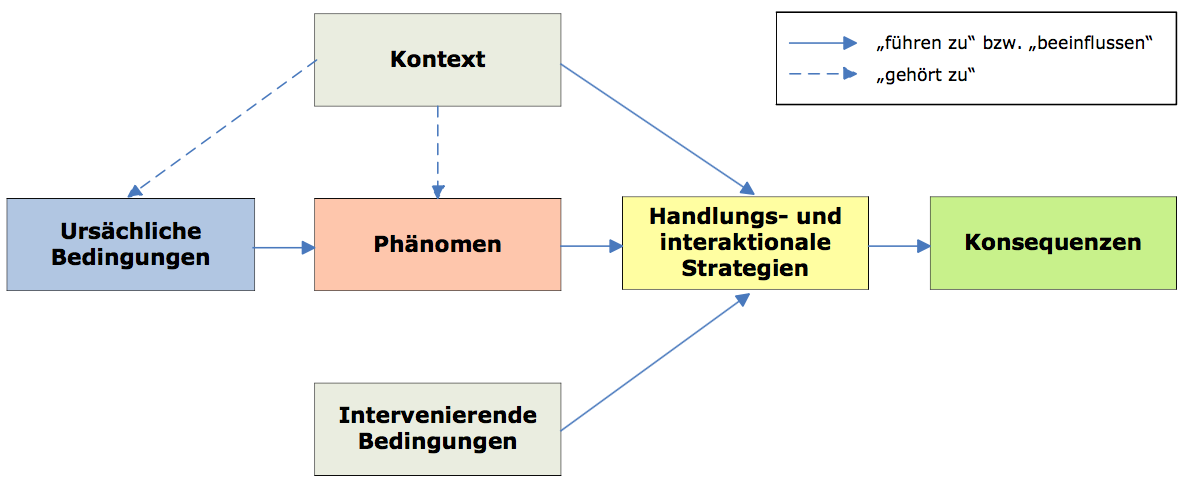
\includegraphics[width=0.75\linewidth]{Figures/paradigmatisches-modell.png}
  \caption[Paradigmatisches Modell]{Paradigmatisches Modell \citep[][S. 67]{Salinger:2013vd}}
  \label{fig:paradigmatisches-modell}
\end{figure}
  
  Vereinfachend technisch ausgedrückt, könnte man das paradigmatische Modell als auseinandersetzungsfördernde Schablone für die Zusammenhänge von Konzepten begreifen. Im Zentrum steht dabei ein Phänomen, auf welches das Handeln gerichtet ist. Bezogen auf dieses Phänomen interessieren dann beispielweise (kausale) ursächliche Bedingungen, eingesetzte Strategien und die Konsequenzen\footnote{Die Bestandteile \textit{Kontext} und \textit{intervenierende Bedingungen} des paradigmatischen Modells sind ein Paradebeispiel für die schlechte Begriffsschärfe, auf die man in der gängigen Literatur trifft. Erst durch \cite{Salinger:2013vd} haben ein Kollege und ich verstanden, worin der genaue Unterschied zwischen \textit{Kontext} und \textit{intervenierende Bedingungen} besteht. Passendere Bezeichner wären für Kontext \textit{spezieller Kontext} und für intervenierende Bedingungen \textit{allgemeiner} oder \textit{breiter Kontext}. Nicht die \textit{intervenierenden Bedingungen}, sondern der \textit{Kontext} ist es, der die ``Ausprägungen der Eigenschaften des im Mittelpunkt der Betrachtung stehenden Phänomens'' beschreibt. Die \textit{intervenierenden Bedingungen} beschreiben lediglich den ``breiteren strukturellen Kontext''.}.
  
  Das paradigmatische Modell hilft dabei, Hypothesen in Beziehung zu setzen, sie zu verifizieren sowie Konzepteigenschaften und Variationen von Phänomenen zu suchen. Man wechselt also stetig zwischen induktivem und deduktivem Denken, was noch einmal im \sref{sec:Erkenntnisperspektive} eine Rolle spielen wird.
  
  In der Literatur scheint es keine Bezeichnung für eine konkrete Ausprägung / Instanz eines paradigmatischen Modells zu geben. Daher führe ich an dieser Stelle den Begriff \textit{\gls{ac}} für Instanzen des paradigmatischen Modells ein, die auf Phänomen-Ebene Zusammenhänge beschreiben. Für Instanzen des paradigmatischen Modells, die auf Konzept-Ebene arbeiten, verwende ich den Begriff \textit{\gls{acm}}.
  
  Geht es dem Forscher lediglich um eine Konzeptentwicklung, genügen offenes und axiales Kodieren.
  
  \item[3. Selektives Kodieren] \hfill \\
  Selektives Kodieren geht über die reine Konzeptentwicklung hinaus und ermöglicht die Entwicklung einer \gls{gt}, was der \gls{gtm} nicht zuletzt ihren Namen gibt. Dabei werden die vorhandenen Erkenntnisse ``systematisch zu einem Bild der Wirklichkeit'' entwickelt.
  
  Im Zentrum steht das zentrale Phänomen, das als \textit{Kernkategorie} bezeichnet wird und gegebenenfalls erst noch entwickelt werden muss. Ähnlich zum axialen Kodieren werden um die \textit{Kernkategorie} ``herum andere Kategorien integriert''. Dieser Prozess sollte mit der Motivation erfolgen, eine \textit{Geschichte} zu erzählen, welche die folgenden Fragen beantwortet:
  
  \begin{itemize}
    \item Was ist im Untersuchungsbereich am auffallendsten?
    \item Welche Phänomene werden wiederholt in den Daten gespiegelt?
    \item Was halte ich für das Hauptproblem?
  \end{itemize}
\end{description}

Zwar werden diese Phasen nicht sequentiell durchlaufen, dennoch ist das offene Kodieren zu Beginn, und das selektive Kodieren gegen Ende der Forschung häufiger zu erwarten.



\subsection{Gütekriterien}

Die \gls{gtm} ist ein ``handlungs- und interaktionsorientiertes Verfahren zur systematischen, qualitativen Analyse von Daten'' \citep{Salinger:2013vd} und unterscheidet sich damit wesentlich von quantitativer Forschung.

Die Gütekriterien quantitativer Forschung können nicht ohne weiteres auf qualitative Forschung übertragen werden. Stattdessen muss die Güte qualitativer Forschungsergebnisse argumentativ nachgewiesen werden. \citep{mayring2002einfhrung}

Im Folgenden fasse ich die sechs allgemeinen Gütekriterien qualitativer Forschung \citep{mayring2002einfhrung} zusammen:
\begin{description}
  \item[Verfahrensdokumentation] Für qualitative Forschung gibt es keine standardisierten Techniken und Messinstrumente, auf die verwiesen werden könnte. Weil qualitative Forschung auf einen Gegenstand bezogen ist, muss das Zustandekommen der Ergebnisse im Detail dokumentiert werden, um den Forschungsprozess für andere nachvollziehbar zu machen.
  
  \item[Argumentative Interpretationsabsicherung] Bei der qualitativen Forschung entstehen die Ergebnisse durch die Interpretationen des Forschers. Um diese adäquat prüfen zu können, müssen sie argumentativ begründet werden. Relevant ist dabei, ob Vorverständnis und Interpretationen des Forschers übereinstimmen. Die Interpretation muss schlüssig, Brüche erklärt und Alternativdeutungen erläutert sein.
  
  \item[Regelgeleitetheit] Trotz der Offenheit qualitativer Forschung muss das Ergebnis systematisch zu Stande kommen. Darauf Bezug nehmend, müssen die einzelnen Analyseeinheiten festgelegt, systematisch und schrittweise bearbeitet sein. Abweichungen von dieser Systematik müssen begründet werden.
  
  \item[Nähe zum Gegenstand] Forschung soll sich nahe am Forschungsgegenstand bewegen und ihr angemessen sein. Dieses Gütekriterium besteht im Nachweis dieser Nähe.
  
  \item[Kommunikative Validierung] Die Gültigkeit der Ergebnisse lässt sich nachweisen, indem diese beispielsweise mit den Beforschten besprochen werden.
  
  \item[Triangulation] Dieses Kriterium macht die Güte des Forschungsergebnisses von den verschiedenen eingesetzten Lösungswegen abhängig. Dazu gehören verschiedene Datenquellen, Interpreten, Theorieansätze und Methoden.
\end{description}

\bigskip

\cite{gesis-solis-00272267} formuliert in ihrem Buch ebenfalls ``Kriterien qualitativer Forschung'', welche die zuvor genannten Gütekriterien anders zusammenfassen. Drei dieser acht Kriterien möchte ich an dieser Stelle nennen, weil sie Aspekte der obigen Kriterien für meine Begriffe treffender bzw. prägnanter gruppieren:

\begin{description}
  \item[Intersubjektive Nachvollziehbarkeit] Die {\raise.17ex\hbox{$\scriptstyle\sim$}} soll eine ``(kritische) Verständigung über eine empirische Studie zwischen Forschern und Lesern'' ermöglichen. Dazu gehört u.a. die Dokumentation des Forschungsprozesses und die Anwendung kodifizierter Verfahren.
  \item[Reflektierte Subjektivität] Da in der qualitativen Forschung der Forscher mit seiner Subjektivität selbst Bestandteil des Forschungsprozesses ist, muss er seine eigene Rolle bei der Theoriebildung reflektieren.
  \item[Limitation] Dieses Kriterium befasst sich mit den Grenzen der Verallgemeinerbarkeit der entwickelten Theorie.
\end{description} 

\bigskip

Die Gütekriterien zeigen, wie stark die Güte qualitativer Forschung von dem Forschenden abhängt. Das ist der Grund, weshalb ich mich entschieden habe, für die Darstellung meiner Arbeit die Ich-Form zu verwenden.




\subsection{Anwendung der Methode der Grounded Theory in dieser Arbeit}

\subsubsection{GTM-Variante}

Für die in dieser Arbeit vorgestellte Forschung habe ich die \gls{gtm} nach \cite{strauss1990basics} im Rahmen einer explorativen, empirischen Fallstudie verwendet. Lediglich die explizite Auffassung von nicht-menschlichen Objekten als Akteure --- zu denen explizit auch Technologien gehören --- habe ich der ``situativen'' \gls{gtm} nach \cite{clarke2005situational} entnommen.

Damit habe ich mich auch gegen die \gls{gtm} nach \cite{glaser1978theoretical} entschieden. Dessen Purismus hat sicherlich seine Berechtigung, jedoch habe ich Zweifel, dass gerade \gls{gtm}-Anfänger in einer überschaubaren Zeit ein hinreichend entwickeltes Ergebnis erzielen.

\subsubsection{Notationen}
\label{sec:notationen}

In dieser Arbeit verfolge ich das methodische Ziel einer hohen Nachvollziehbarkeit. Zu diesem Zweck vereinbare ich folgende Notationen:

\begin{itemize}\raggedright
  \item Kodes, Konzepte und Kategorien werden wie folgt notiert: \code{Bezeichner}
  \begin{itemize}
    \item Beispiel: \code{apiua://code/-9223372036854775615}
    \item Diese Darstellung wird durch das \texttt{\textbackslash{}code}-Makro erzeugt, das Bestandteil meines \LaTeX-Pakets \texttt{apiua} ist. Das Beispiel wurde durch den Befehl \textbackslash{}code\{apiua://code/-9223372036854775615\} konstruiert.  
    \item Der Bezeichner ist verlinkt und verweist eindeutig auf das entsprechende Element innerhalb meiner Forschungsdaten. Im angezeigten Beispiel lautet die URI \url{apiua://code/-9223372036854775615}.
    \item Da zur Auflösung der Links eigentlich das im \sref{sec:apiua} beschriebene Datenanalysewerkzeug installiert sein muss, verweisen die Links stattdessen auf eine ebenfalls öffentlich zugängliche HTML-Fassung meiner Forschungsdaten.
    \item Das HTML-Dokument listet alle gefundenen Kodes/Konzepte/Kategorien/Relationen hierarchisch auf. Zu jedem Eintrag wird mein Memo und alle von mir entdeckten Phänomene (\textit{Instances}) dargestellt. Eventuell vorhandene Memos in Bezug auf einzelne Phänomene werden ebenfalls angezeigt. Häufig verfügen abstrakte Kodes nicht über unmittelbare Phänomene. In diesem Fall empfiehlt es sich, die Phänomene von Unterkodes zu betrachten.
  \end{itemize}
  
  \item Relationen werden wie folgt notiert: \rel[Name]{\code{Bezeichner 1}}{\code{Bezeichner 2}}
  \begin{itemize}
    \item Beispiel: \mbox{\rel[f"uhren\ zu]{\code[apiua://code/-9223372036854775281]{Intuitive Entwurfsentscheidungen}}{\code[apiua://code/-9223372036854774939]{Usability-Problemen}}}
    \item Unbenannte Relationen haben das Format: \mbox{\rel{\code{Bezeichner 1}}{\code{Bezeichner 2}}}
    \item Die Elemente einer Relation sind ebenfalls verlinkt.
  \end{itemize}
  
  \item Wichtigkeit wird durch Opazität notiert: \codebullet{apiua://code/-9223372036854774814}\,\codebullet{apiua://code/-9223372036854774813}\,\codebullet{apiua://code/-9223372036854774812}
  \begin{itemize}
    \item Standardmäßig wird ein semi-transparenter Kreis (\codebullet{apiua://code/-9223372036854774813}) verwendet.
    \item Ein vollfarbiger Kreis (\codebullet{apiua://code/-9223372036854774814}) markiert besonders wichtige Kodes, Konzepte und Kategorien.
    \item Ein transparenter Kreis (\codebullet{apiua://code/-9223372036854774812}) markiert weniger wichtige Kodes, Konzepte und Kategorien.
    \item Die verwendeten Farben geben Aufschluss über die Zusammengehörigkeit von Kodes, Konzepten und Kategorien. Deren Zusammengehörigkeit wird durch ähnliche Farben gekennzeichnet.
  \end{itemize}
  
  \item Zitate der von mir erfassten Rohdaten sind mit dem Open-Access-Symbol versehen: \raisebox{-0.3ex}{
\includegraphics[height=2.2ex]{Figures/openaccess.pdf}} %\textsuperscript{$\star$}
  \begin{itemize}
    \item Beispiel: ``to make things more funny there are places in SeqAn where the subscript operator returns values and not references''\citepurl{apiua://groupDiscussion/workshop\%2712+-+Interview+Gruppendiskussion+\%282012-09-06T13-01-28\%2B0200\%29.html/li/59}
    \item Das Open-Access-Symbol ist mit dem entsprechenden, öffentlich zugänglichen Rohdatum verlinkt, wie dies auch bei Kodes, Konzepten und Kategorien der Fall ist.
  \end{itemize}
  
  \item Bezeichnungen mit einem Glossar-Eintrag verfügen über ein hochgestelltes ``G'': \textsuperscript{\textsuperscript{\tiny G}}
  \begin{itemize}
    \item Beispiel: \gls{euse}
    \item Annotiert sind je Kapitel nur die ersten Vorkommnisse.
    \item Jedes Vorkommnis ist mit dem entsprechenden Glossar-Eintrag verlinkt.
  \end{itemize}
\end{itemize}

\begin{comment}
\begin{description}
  \item[Kodes / Konzepte / Kategorien] \hfill \code{Bezeichner}
  
  Der Bezeichner ist verlinkt und verweist auf das tatsächliche Element innerhalb der Forschungsdaten. In den Forschungsdaten sind die Datenpunkte/Phänomene zu finden, auf denen das Element basiert.
  
  Beispiel: \code{apiua://code/-9223372036854775615}
  
  \bigskip
  
  \item[Relationen] \hfill \rel[Name]{\code{Bezeichner 1}}{\code{Bezeichner 2}}
  
  Beispiel: \rel[f"uhren\ zu]{\code[apiua://code/-9223372036854775281]{Intuitive Entwurfsentscheidungen}}{\code[apiua://code/-9223372036854774939]{Usability-Problemen}}
  
  \bigskip
  
  \item[Farben] \hfill \codebullet{apiua://code/-9223372036854774814}\,\codebullet{apiua://code/-9223372036854774813}\,\codebullet{apiua://code/-9223372036854774812}
  
  Die Farben geben Aufschluss über die Zusammengehörigkeit von Konzepten und werden durch einen semi-transparenten Kreis (\codebullet{apiua://code/-9223372036854774813}) dargestellt. Ein vollfarbiger Kreis (\codebullet{apiua://code/-9223372036854774814}) markiert besonders wichtige und ein transparenter Kreis (\codebullet{apiua://code/-9223372036854774812}) weniger wichtige Konzepte.
\end{description}
\end{comment}



\subsubsection{Gliederung}

Obwohl klassisches, aus der quantitativen Forschung bekanntes Vorgehen nicht die Idee der \gls{gtm} ist, werden Teile dieser Arbeit so gegliedert, wodurch ich lediglich das Lesen erleichtern möchte. Tatsächlich sind aber viele Tätigkeiten parallel verlaufen.

So stelle ich meine im \hyperref[sec:forschung]{Kapitel 3} vorgestellte Forschung in sequentiellen Phasen dar, welche sich tatsächlich aber überlappt und teilweise auch gegenseitig stark beeinflusst haben. Die zeitaufwändige erste Beseitigung ``grober'', teils offensichtlicher Usability-Probleme reichte in die eigentliche \gls{gtm}-Forschung hinein, die wiederum im stetigen Wechsel zur Entwicklung eines eigens für meine Forschung entwickelten qualitativen Analysewerkzeugs stand.

Bevor ich jedoch meine Forschung vorstelle, gebe ich im nächsten Kapitel zunächst eine umfassende Literaturübersicht. Diese Literaturübersicht habe ich nicht zu Beginn meiner Forschung, sondern erst ein Jahr später erarbeitet. Auf diese Weise konnte ich meinem Anspruch an eine explorative Studie gerecht werden und einen sensiblen Umgang mit bestehender Literatur erreichen.


 
\cleardoublepage